\documentclass[11pt,a4paper]{report}
\usepackage[utf8]{inputenc}
\usepackage[french]{babel}
\usepackage[T1]{fontenc}
\usepackage{amsmath}
\usepackage{amsfonts}
\usepackage{amssymb}
\usepackage{xcolor}

\usepackage{geometry}
\geometry{hmargin=2.5cm,vmargin=1.5cm}
\usepackage{wasysym}
\usepackage{graphicx}

\author{Mathieu Sarrat}
\title{LP13 - Ondes progressives et ondes stationnaires}

\makeatletter
\renewcommand{\thesection}{\@arabic\c@section}
\makeatother


\begin{document}
\maketitle

\section{Introduction}

Lorsqu'on perturbe une eau calme, par exemple en y jetant une pierre, l'eau s'agite : on observe autour de la zone d'impact la formation de rides circulaires qui s'agrandissent au cours du temps [MANIP ou images]. On dit qu'il se forme des ondes à la surface de l'eau : la perturbation créée par la pierre semble se propager.\\

Dans notre vie quotidienne, les ondes servent essentiellement à communiquer et à transmettre une information. Et pour cause, nous percevons l'expérience précédente de deux façons : à travers l'ouïe et à travers les yeux. Le bruit produit par la chute de la pierre dans l'eau se propage de la zone d'impact à nos oreilles sous forme de son (ondes acoustiques). Si nous voyons la pierre tomber et l'eau se déformer, c'est parce que la pierre et l'eau nous renvoient de la lumière et que nos yeux captent cette lumière. On sait depuis le $\text{XIX}^\text{e}$ siècle et les travaux de Maxwell et Hertz que la lumière a une nature ondulatoire, qu'elle est une onde électromagnétique. Ces dernières sont extrêmement utilisées pour transporter des informations sur de très longues distances, pour un coût relativement peu onéreux : la radio, les téléphones mobiles.\\

Dans cette leçon nous allons introduire les notions d'onde et de propagation et les illustrer en nous appuyant sur un exemple précis, celui de la \textbf{corde de Melde}. 

\section{Définition d'une onde}\label{sec:1}

\subsection{Mise en évidence}

Soit une corde \ref{fig:corde_melde} dont une extrémité est reliée à une source de vibration (commandée par un GBF) et dont l'autre extrémité est liée à une masse $m$. La source de vibration impose un ébranlement (mouvement transversal quelconque) au point O. On suppose que la masselotte $m$ impose une tension $T = mg$ dans toute la corde.\\

\begin{figure}[h!]
\begin{center}
	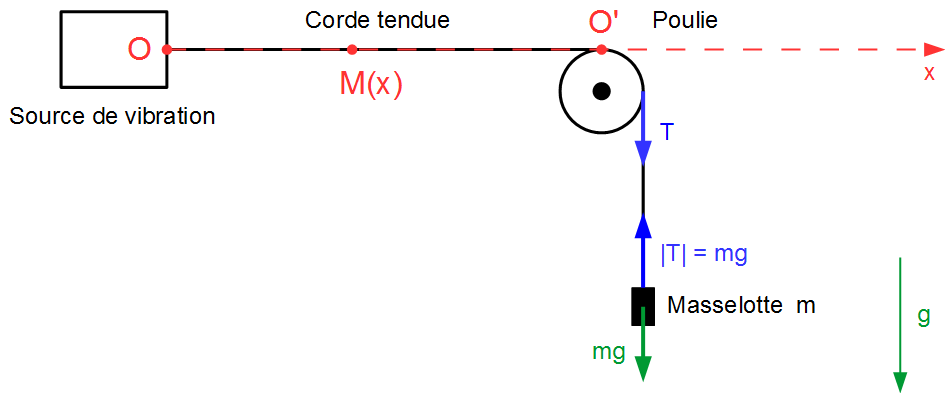
\includegraphics[scale = 0.5]{corde_melde.png}
	\caption{Corde de Melde} 
	\label{fig:corde_melde}
\end{center}
\end{figure}

\begin{figure}[h!]
\begin{center}
	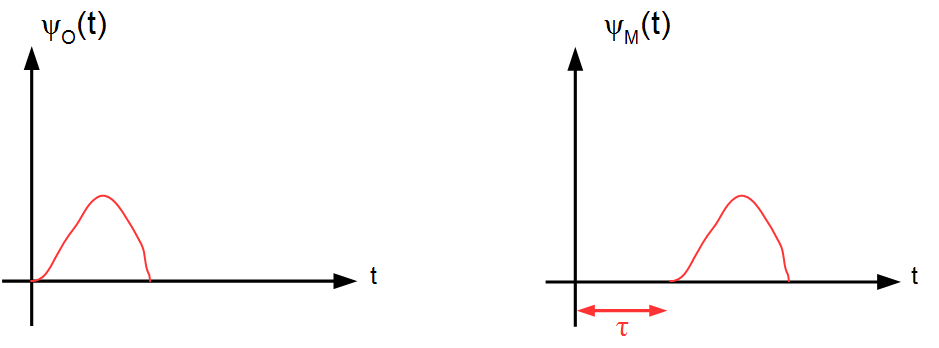
\includegraphics[scale = 0.5]{propagation.png}
	\caption{Propagation d'une perturbation} 
	\label{fig:propagation}
\end{center}
\end{figure}

Le signal émis au point O peut être décrit par une fonction du temps $\Psi_O$. On constate qu'à un instant $\tau$ (appelé \textbf{retard}), le point M situé à la distance $x$ de O acquiert le même mouvement \ref{fig:propagation} : il y a propagation vers les $x$ croissants et M perçoit le même signal que O mais décalé dans le temps. Le signal en $x$ à l'instant $t$, $\Psi_M(t) \equiv \Psi(x,t)$, est le même que celui au point O à l'instant $t-\tau$, d'où
\begin{equation}
	\Psi(x,t) = \Psi_O(t-\tau).
\end{equation} 
\textit{On a supposé qu'il n'y avait ni déformation, ni atténuation du signal, ce qui peut se produire si la corde est trop longue ou que sa raideur n'est pas négligeable.}\\

On observe que le retard $\tau$ est proportionnel à la distance $x$ parcourue par la perturbation. On peut écrire 
\begin{equation}
	\tau = \frac{x_1 - x_0}{v}
\end{equation}
où $v$ désigne la \textbf{vitesse de propagation de l'onde} (également appelée \textbf{célérité}) ou encore, comme nous le verrons plus loin, sa \textbf{vitesse de phase}.

Dans ce cas, le signal perçu au point M s'écrit
\begin{equation}
	\Psi(x,t) = \Psi_O(t-\frac{x}{v}) \equiv \Psi_+(t-\frac{x}{v}),
\end{equation} 
où le signe $+$ rappelle que la propagation se fait dans le sens des $x$ croissants.\\

Expérimentalement, on montre que
\begin{equation}
	v = \sqrt{\frac{T}{\mu}}
\end{equation}
où $T$ désigne la tension de la corde (la force exercée par un morceau de corde sur le morceau voisin) et $\mu$ sa masse linéique. \textbf{De façon générale, les ondes mécaniques se propagent d'autant plus mal que le milieu est mou et inerte.} Pour une corde de piano en acier \textcolor{red}{[vérifier matériau... peut-être du nylon]}, de diamètre $d = 0.8 mm$ et de masse volumique $\rho = 7200\;\text{kg}.\text{m}^{-3}$, on trouve $\mu = \rho \pi \frac{d^2}{4} = 3.6 \times 10^{-3}\;\text{kg}.\text{m}^{-1}$. La corde est tendue par la masselotte $m = 0.2\;\text{kg}$, sa tension est donc, en valeur absolue $T = mg$, d'où
\begin{equation}
	v = \left(\frac{0.2\times 9.81}{3.6 \times 10^{-3}}\right)^{\frac{1}{2}} \simeq\;23 \text{m}/\text{s}.
\end{equation}

\subsubsection{Propagation dans les deux sens}

La corde étant fixée en O', on observe que, lorsque l'ébranlement atteint O', apparaît une onde réfléchie qui se propage selon le sens des $x$ décroissants. Cette onde régressive peut être représentée par une élongation
\begin{equation}
	\Psi(x,t) \equiv \Psi_-\left(t + \frac{x}{v}\right).
\end{equation}
On constate une inversion du sens de propagation, d'où $x$ transformé en $-x$ dans l'expression de l'onde.

\subsubsection{Propagation sans transport de matière}

Après le passage de l'onde, les points O et M retrouvent leur position d'origine, ils ne sont pas déplacés : il y a donc transport d'information (puisque la perturbation, c'est à dire la forme de la corde, se propage) mais pas transport de matière. La grandeur perturbée lors du passage de l'onde (ici l'élongation transverse de la corde) s'écrit comme une \textbf{fonction de deux variables} : le temps et l'espace. C'est une caractéristique de tout phénomène propagatif.
 
\subsection{Définition}

Une \textbf{onde} est le phénomène physique correspondant à la \textbf{propagation d'information, sans transport de matière mais avec transport d'énergie}, d'un point
à un autre \textbf{par les seules variations locales de champs} scalaires (ex : pression, pour les ondes sonores) ou vectoriels (ex : $(\bold{E},\bold{B})$ pour les ondes électromagnétiques) fonctions du point M et de l'instant t.

\subsection{\'Equation de propagation}

\subsubsection{Problème à une dimension spatiale}

Pour divers problèmes de physique des ondes (acoustique, lumière dans le vide, corde vibrante ... )la grandeur physique $\Psi(x,t)$ porteuse d'une information est solution d'une même équation d'onde appelée équation de de propagation ou encore \textbf{équation de d'Alembert} (du nom de celui qui l'a écrite pour la première fois). Nous allons établir cette équation dans le cas de la corde tendue.\\

\begin{figure}[h!]
\begin{center}
	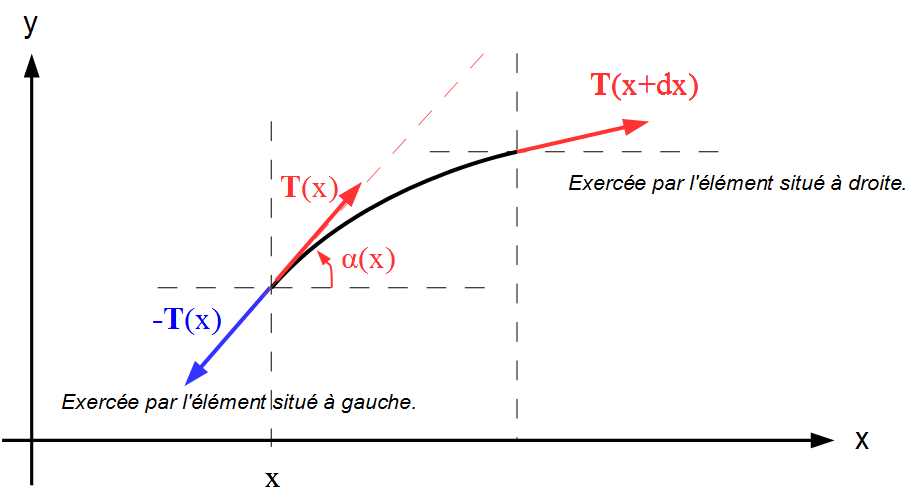
\includegraphics[scale = 0.5]{corde_tendue.png}
	\caption{Modèle de propagation dans une corde.} 
	\label{fig:corde_tendue}
\end{center}
\end{figure}

Nous nous plaçons sous les hypothèses suivantes :
\begin{itemize}
	\item la corde est filiforme, de masse linéique constante et de longueur $L_0$;
	\item son poids est négligeable : à l'équilibre, la corde est horizontale;
	\item la corde est \textbf{infiniment souple} : sa raideur est nulle, elle transmet donc sur toute sa longueur une force de tension $T$ constante en module, parallèle à la corde en chacun de ses points;
	\item la corde est \textbf{parfaitement élastique} : son étirement $e$ est proportionnel à la tension $T$, parfaitement réversible et sans perte d'énergie par frottement interne 
	($T = Ke$, où $K$ module d'élasticité constant. Loi de Hooke simplifié);	
	\item on ne s'intéresse qu'à une \textbf{onde purement transversale} : déformations dans la direction $y$ seulement (on néglige les vibrations longitudinales et de torsion);
	\item la perturbation causée par la propagation de l'onde est de faible ampleur : \textbf{faibles déformations selon $y$}. Si on désigne par $\alpha(x)$ l'angle entre l'horizontale et la tangente à la corde au point $x$, cet angle est lui aussi très petit. Dans ce cas :
	\begin{equation}
		\text{cos}\;\alpha \simeq 1 \qquad\text{et}\qquad \text{sin}\;\alpha \simeq \alpha,
	\end{equation}
	et
	\begin{equation}
		\alpha \simeq \text{tan}\;\alpha \simeq \frac{\partial y}{\partial x}
	\end{equation}
	à l'ordre $1$.
\end{itemize}
Une telle corde n'existe évidemment pas dans la réalité, mais elle simule assez bien les cordes utilisées par exemple dans les instruments de musique.\\

Soit un élément de cette corde, de longueur $d\ell$ et de masse $\mu d\ell$. Comme on \textbf{néglige le poids}, seules deux forces s'exercent donc sur $d\ell$ :
\begin{itemize}
	\item la tension exercée par l'élément de corde situé au-delà de $x+dx$, notée $\bold{T}(x+dx,t)$,
	\item la tension exercée par l'élément de corde situé en-deçà de $x$, notée $-\bold{T}(x,t)$ (d'après la troisième loi de Newton).
\end{itemize}
La corde étant \textbf{infiniment souple}, ces deux forces sont égales en module quelque soit le mouvement communiqué à la corde. Ainsi :
\begin{equation}
	|\bold{T}(x+dx,t)| = |\bold{T}(x,t)| = T. 
\end{equation} 

Au repos, ces forces se compensent. Lors du passage de l'onde, la corde s'éloigne de sa position d'équilibre et les forces de tension ne se compensent plus, mais leur norme reste la même (imposée par la masselotte, et transmise parfaitement du fait de l'infinie souplesse de la corde). On décrit l'élongation de la corde par la position de chaque élément la constituant selon l'axe y à chaque instant: $\bold{r}(x,t) \equiv \Psi(x,t)$. La loi fondamentale de la dynamique s'écrit :
\begin{equation*}
	\mu d\ell \frac{\partial^2 \bold{r}}{\partial t^2} = \bold{T}(x+dx,t) - \bold{T}(x,t) = \frac{\partial \bold{T}}{\partial x} dx.
\end{equation*}
La déformation étant faible, $d\ell \simeq dx$, d'où
\begin{equation}
	\mu \frac{\partial^2 \bold{r}}{\partial t^2} = \frac{\partial \bold{T}}{\partial x}.
\end{equation}

On peut ensuite écrire 
\begin{equation}
	\bold{T}(x) = T \text{cos}\;\alpha(x)\bold{e}_x  + T \text{sin}\;\alpha(x)\bold{e}_y,
\end{equation}
d'où 
\begin{align*}
	\frac{\partial \bold{T}}{\partial x} & = T \frac{\partial}{\partial x}\left[\text{cos}\;\alpha(x)\bold{e}_x + \text{sin}\;\alpha(x)\bold{e}_y \right]\\
	& = T \frac{\partial \alpha}{\partial x}\left[-\text{sin}\;\alpha \bold{e}_x  +  \text{cos}\;\alpha \bold{e}_y\right]\\
	& = T \frac{\partial \alpha}{\partial x}\left[-\alpha \bold{e}_x  + \bold{e}_y\right]\\
	& = T \frac{\partial}{\partial x}\left(\frac{\partial y}{\partial x}\right)\left[-\alpha \bold{e}_x  + \bold{e}_y\right] 
	= T\frac{\partial^2 y}{\partial x^2}\left[-\alpha \bold{e}_x  + \bold{e}_y\right],
\end{align*}
où l'on a utilisé les développements limités de cos, sin et tan à l'ordre 1, comme expliqué plus haut.\\

Comme l'onde est purement transversale,
\begin{equation}
	\frac{\partial^2 \bold{r}}{\partial t^2} = \frac{\partial^2 y}{\partial t^2}
\end{equation}
d'où, en projetant selon $y$ :
\begin{equation*}
	\mu \frac{\partial^2 y}{\partial t^2} =  T\frac{\partial^2 y}{\partial x^2}.
\end{equation*}

En réarrangeant les termes, on obtient l'\textbf{équation de d'Alembert} :
\begin{equation}
	\frac{\partial^2 y}{\partial x^2} - \frac{1}{v^2}\frac{\partial^2 y}{\partial t^2} = 0,
\end{equation}
avec $v = \sqrt{T/\mu}$ comme attendu. Rappelons que $T = mg$ en tout point de la corde, compte tenu de la souplesse de celle-ci et de la masselotte attachée à l'une de ses extrémités. On remarquera que l'équation précédente traduit la réversibilité dans le temps de la transformation correspondant à la propagation de l'onde, puisqu'elle est invariante si on transforme $t$ en $-t$ : ceci est logique puisque nous avons négligé tout effet d'amortissement.\\

\textbf{Remarque :} la projection selon $\bold{e}_x$ conduit à
\begin{align*}
	0 & = \frac{\partial \bold{T}}{\partial x}\cdot\bold{e}_x = \left[\frac{\partial T}{\partial x} \text{cos}\;\alpha + T(x)\frac{\partial}{\partial x} \text{cos}\;\alpha \right]\\
	& = \left[\frac{\partial T}{\partial x} \text{cos}\;\alpha - T(x)\text{sin}\;\alpha \frac{\partial \alpha}{\partial x}\right].
\end{align*}
Le dernier terme est non-linéaire (relatif à $\alpha^2$) : il est donc négligé et négligeable tant que $\alpha$ est suffisamment petit. Sous cette hypothèse (qui n'est rien d'autre que celle des faibles perturbations), on trouve
\begin{equation}
	0 \simeq \frac{\partial T}{\partial x},
\end{equation}
qui est une réécriture de l'hypothèse de la corde infiniment souple.

\subsubsection{Généralisations}

Dans le cas de l'espace à trois dimensions, l'équation de d'Alembert prend la forme suivante,
\begin{equation}
	\Delta \Psi = \frac{1}{v^2} \frac{\partial^2\Psi}{\partial t^2},
\end{equation}
où $\Delta$ est l'opérateur Laplacien. Cet opérateur est une généralisation à trois dimensions de la dérivée seconde par rapport à la variable d'espace $x$. Ainsi, les ondes sonores dans un fluide ($\Psi$ est la pression du fluide) ou la lumière (approximation de l'optique ondulatoire) peuvent se propager dans toutes les directions de l'espace à partir de sources plus ou moins ponctuelles.\\

Enfin, la variable perturbée représentée par la fonction d'onde $\Psi$ n'est pas nécessairement scalaire. La propagation d'une onde électromagnétique dans le vide (la lumière), loin de toute source de champ, est décrite par l'équation d'Alembert et c'est le champ électromagnétique $(\bold{E},\bold{B})$ qui tient le rôle de $\Psi$. Ces divers exemples d'ondes feront l'objet de leçons, voire de cours, ultérieurs.

\newpage
\section{Ondes progressives}\label{sec:2}

De façon générale, si les équations décrivant le comportement d'un système se combinent en conduisant à une équation d'onde, c'est que des ondes peuvent se propager dans le milieu étudié. Nous allons nous intéresser dans cette section aux ondes progressives (qui se propagent).

On appelle \textbf{onde progressive} un phénomène physique caractérisé par une grandeur dont la variation dans le temps et l'espace dépend de la quantité
\begin{equation}
	t \pm \frac{x}{v},
\end{equation}
mise en évidence dans la première partie de cette leçon. On retiendra que lorsque la propagation a lieu \textbf{selon les $x$ croissants}, les variables \textbf{$x$ et $t$ sont affectées de signes opposés}.

\subsection{Solution générale de l'équation de propagation}

Il existe plusieurs types de \textbf{solutions} progressives à l'équation de d'Alembert
\begin{equation}
	\Delta \Psi - \frac{1}{v^2} \frac{\partial^2\Psi}{\partial t^2} = 0.
\end{equation}

On en distingue deux qui sont conceptuellement importantes :
\begin{itemize}
	\item les \textbf{ondes sphériques}, caractérisées par $\Psi(r,t)$ où $r$ est la distance entre le point M recevant l'onde et la source ponctuelle O. \'A tout instant, l'état vibratoire (et donc la valeur de $\Psi$) est le même en tout point d'une sphère de centre 0 et de rayon $r$. La solution correspondante de l'équation de d'Alembert est de la forme
	\begin{equation}
		\Psi = \frac{1}{r}\mathcal{S}_+\left(t - \frac{x}{v}\right) + \frac{1}{r}\mathcal{S}_-\left(t + \frac{x}{v}\right),
	\end{equation}
	où $\mathcal{S}_+$ et $\mathcal{S}_-$ sont imposées par la source. Le premier terme décrit une onde qui diverge depuis le centre de la sphère, la second une onde qui converge vers son centre (dans ce cas la source ne se trouve pas à cet endroit). On remarque la dépendance en $1/r$ de la fonction d'onde, qui traduit une atténuation.\\ 

	\item les \textbf{ondes planes}, caractérisées par une surface d'onde plane : la valeur de $\Psi$ est la même en tout point d'un plan s'il est perpendiculaire à la direction de propagation OX. Soit un tel plan, de vecteur normal $\bold{e}_X$ qui désigne la direction de propagation de l'onde et un point M repéré par $\bold{r}$. Tous les points vérifiant l'équation
	\begin{equation}
		\bold{e}_X\cdot\bold{r} = \text{Cte}
	\end{equation}	 
	appartiennent à un même plan. Dans ce cas, la fonction d'onde ne dépend que de $t$ et de $\bold{e}_X\cdot\bold{r}$, d'où l'expression générale d'une onde plane solution de l'équation de d'Alembert
	\begin{equation}
		\Psi(x,t) = \Psi_+\left(t - \frac{\bold{e}_X\cdot\bold{r}}{v}\right) + \Psi_-\left(t + \frac{\bold{e}_X\cdot\bold{r}}{v}\right).
	\end{equation}
	Ce modèle très idéal permet cependant de décrire le cas d'une onde sphérique divergente reçue par une petite surface et qui est observée assez loin de sa source. C'est aussi une bonne 		façon de décrire la lumière sortant d'une lentille convergente lorsque sa source se trouve sur le foyer objet de cette lentille. Pour ces deux raisons notamment, le modèle de l'onde 			plane est souvent utilisé.
\end{itemize} 

Dans le problème plus simple de la corde de Melde, ou nous avons souligné la possibilité pour une onde de se propager selon deux sens, la solution générale de l'équation de d'Alembert
\begin{equation}
	\frac{\partial^2 \Psi}{\partial x^2} - \frac{1}{v^2}\frac{\partial^2 \Psi}{\partial t^2} = 0,
\end{equation}
s'écrit 
\begin{equation}
	\Psi(x,t) = \Psi_+\left(t - \frac{x}{v}\right) + \Psi_-\left(t + \frac{x}{v}\right).
\end{equation}	
La première fonction traduit une propagation vers les $x$ croissants et la seconde une propagation vers les $x$ décroissants. Ceci est vrai dans un espace à une dimension, comme la corde. On peut dire que l'onde se propageant dans la corde est une onde plane (et ce malgré le caractère filiforme du modèle) car la corde a une section qui est petite mais non nulle.

\subsection{Onde plane progressive monochromatique}

Nous allons nous intéresser maintenant à un cas particulier très important. On appelle \textbf{onde plane progressive monochromatique} (OPPM) une onde dont la fonction d'onde s'écrit
\begin{equation}
	\Psi\left(\bold{r},t\right) = A \text{cos}\left[\omega\left(t - \frac{\bold{e}_X\cdot\bold{r}}{v}\right) - \phi \right] = A \text{cos}\left(\omega t - \bold{k}\cdot\bold{r} - \phi\right),
\end{equation}
où
\begin{equation}
	\omega t - \bold{k}\cdot\bold{r} - \phi
\end{equation}
désigne \textbf{la phase de l'onde} et où
\begin{itemize}
	\item $A$ désigne l'\textbf{amplitude} de l'onde;
	\item $\omega$ (en rad.$\text{s}^{-1}$) est la \textbf{pulsation};
	\item $\bold{k} = \displaystyle{\frac{\omega}{v}}\bold{e}_X$ est le \textbf{vecteur d'onde} en $\text{m}^{-1}$, dirigé selon la \textbf{direction de propagation} et orienté dans le sens de propagation de l'onde. Le signe de $k$ donne le \textbf{sens de propagation};
	\item $\phi$(en rad) est la \textbf{phase à l'origine} (des temps et de l'espace), une constante.
\end{itemize}

On parle d'onde monochromatique car elle oscille à une fréquence bien déterminée, $f = \frac{\omega}{2\pi}$, mesurée en $Hz$ (ou en $\text{s}^{-1}$).\\

\subsubsection{Double-périodicité}

La fonction $\Psi$ caractérisant une OPPM est \textbf{périodique dans le temps et dans l'espace} :
\begin{itemize}
	\item périodicité temporelle :
	\begin{equation}
		\Psi(\bold{r},t) = \Psi(\bold{r},t+T)
	\end{equation}	 
	où $T \equiv 2\pi /omega = 1/f$ (en s) est la période temporelle;
	\item périodicité spatiale :
	\begin{equation}
		\Psi(\bold{e}_X\cdot\bold{r},t) = \Psi(\bold{e}_X\cdot\bold{r} + \lambda,t)
	\end{equation}
	où $\lambda = 2\pi/|\bold{k}|$ (en m) est la \textbf{longueur d'onde} ou période spatiale.
\end{itemize}

Les deux périodes sont liées par la relation
\begin{equation}
	\lambda = 2\pi\frac{v}{\omega} = v T. 
\end{equation}

\textcolor{red}{[Faire un schéma pour illustrer la double périodicité]}

\subsubsection{Vitesse de phase}

Pour une OPPM, les surfaces de même valeur de phase (ou surface d'onde) sont des plans perpendiculaires à $\bold{k}$. Du fait de la propagation, les surfaces d'onde se déplacent avec une vitesse donnée. Considérons un problème à une dimension spatiale (par exemple la corde vibrante). Rappelons que la phase s'écrit :
\begin{equation}
	\Phi = \omega t - k x,
\end{equation}
Dans le cas d'une propagation suivant $x$, la vitesse de cette surface 'équiphase' vérifie
\begin{equation}
	d\Phi = 0 \qquad\text{d'où}\qquad \omega dt - k dx = 0
\end{equation}
équation que l'on peut réécrire
\begin{equation}
	\frac{dx}{dt} = \frac{\omega}{k}.
\end{equation}

La vitesse de phase est par définition
\begin{equation}
	v_\phi \equiv \frac{\omega}{k}.
\end{equation}
Comme $x$ représente la position de la surface équiphase au cours du temps, la vitesse de phase est bien la vitesse avec laquelle se déplace une surface d'onde d'OPPM.

\textit{Remarque : une onde plane progressive monochromatique voit sa vitesse de phase et sa vitesse de groupe être égales. Pour une onde parfaitement sinusoïdale, la vitesse de déplacement du maximum de la vague est égal à ces deux vitesses. Lorsque l'onde n'est pas sinusoïdale monochromatique, vitesse de phase et vitesse de groupe sont distinctes. La vitesse de groupe est la vitesse de transport de l'énergie et correspond à la vitesse de déplacement de l'enveloppe de l'onde.}

\subsubsection{Linéarité, nombres complexes et utilité des ondes planes}

L'équation de d'Alembert est une équation linéaire, c'est à dire que si $f_1(x,t)$ et $f_2(x,t)$ sont solutions de cette équation, alors 
\begin{equation}
	\lambda_1 f_1(x,t) + \lambda_2 f_2(x,t)
\end{equation}
où $\lambda_1$ et $\lambda_2$ sont deux constantes est également solution.\\

Ainsi, la fonction d'onde
\begin{equation}
	\underline{\Psi}(x,t) = A\; \text{cos}\left(\omega t - kx - \phi\right) + i A\; \text{sin}\left(\omega t - kx - \phi\right) = A\text{e}^{i\left(\omega t - kx - \phi\right)}
\end{equation}
telle que $\Psi = \Re(\underline{\Psi})$ est aussi solution de l'équation de d'Alembert. Travailler dans le plan complexe permet souvent de faciliter les calculs. Il faut cependant garder à l'esprit que la solution physique est donnée par la partie réelle de la solution complexe.\\

Les dérivées partielles de $\underline{\Psi}$ s'écrivent :
\begin{equation}
	\frac{\partial \underline{\Psi}}{\partial t} = i\omega\underline{\Psi} \qquad\text{et}\qquad \frac{\partial \underline{\Psi}}{\partial x}  = -ik\underline{\Psi}.
\end{equation}
Pour la corde, l'équation de d'Alembert devient :
\begin{equation}
	\left(- k^2 + \frac{\omega^2}{v^2}\right)\underline{\Psi} = 0.
\end{equation}
On en déduit la \textbf{relation de dispersion} des ondes transversales se propageant dans la corde
\begin{equation}
	\omega^2 = k^2 v^2,
\end{equation}
ce qui implique
\begin{equation}
	k = \pm \frac{\omega}{v} \qquad \text{ou encore}\qquad \omega = \pm k v.
\end{equation}

Une relation de dispersion est une équation permettant de relier la longueur d'onde d'une onde existant dans le milieu étudié à sa fréquence en tenant compte des caractéristiques du milieu (ici la tension de la corde et sa masse linéique). Les relations de dispersion peuvent avoir des expressions bien plus compliquées que celle que nous venons d'obtenir, en fonction des effets physiques que l'on a introduits dans le modèle. Dans le cas de la corde vibrante, pour une fréquence donnée, la relation de dispersion admet deux solutions (deux valeurs de $k$) correspondant à une propagation selon les $x$ croissants ($+$) ou décroissants ($-$).\\

On remarque que $v_\phi = v$, ce qui montre bien que la vitesse de propagation intervenant dans l'équation de d'Alembert est la vitesse de phase. Dans le cas de la corde vibrante, cette vitesse correspond à la vitesse de déplacement du maximum d'amplitude le long de la corde. Il est important de souligner que cette vitesse \textbf{ne caractérise pas nécessairement un déplacement de matière ou un déplacement d'énergie} : ce n'est que la vitesse de propagation de la perturbation. En effet, dans la corde la matière se déplace transversalement alors que l'onde se propage le long de la corde. Il arrive ainsi de rencontrer des vitesses de phase supérieures à celle de la lumière sans que cela ne constitue une violation de la théorie de la relativité.\\

La portée de cette analyse dépasse le cas très particulier de la propagation d'une onde plane, objet idéal n'existant pas réellement. \textbf{Tout signal} périodique $f(x,t)$ à valeurs complexes ou réelles \textbf{peut être représenté comme une somme de fonctions sinusoïdales monochromatiques, c'est à dire d'OPPM} : c'est un développement en série de Fourier. Ainsi, bien que la réalité physique des ondes planes monochromatiques soit discutable \textbf{(une OPPM a une étendue infinie dans le temps et dans l'espace)}, elles sont très utiles puisque tout signal peut rigoureusement être représenté comme une superposition d'OPPM : étudier le comportement d'ondes planes dans le système est donc essentiel. Ce résultat s'étend aux signaux non périodiques grâce à la transformation de Fourier, applicable pour toute fonction à valeur réelle ou complexe intégrable sur le domaine des nombres réels. 

%\subsubsection{Paquet d'ondes et vitesse de groupe (facultatif)}
%
%Ainsi, tout "paquet d'ondes" (comprendre par là une onde équivalente à une somme d'OPPM de fréquences différentes), peut s'écrire sous la forme d'une intégrale de Fourier :
%\begin{equation}
%	\Psi(x,t) = \int_{-\infty}^{+\infty} \int_{-\infty}^{+\infty} \widehat{\Psi}(k,\omega) \text{e}^{j(\omega t - kx)} dk d\omega.
%\end{equation}
%Cette expression correspond bien à une somme d'OPPM. La fonction $\widehat{\Psi}(k,\omega)$ est la transformée de Fourier de la fonction d'onde $\Psi(x,t)$ (qui est elle-même la transformée inverse de $\widehat{\Psi}(k,\omega)$.\\
%
%Dans la plupart des milieux matériels, la vitesse de propagation dépend de la fréquence : on parle de milieu dispersif et dans ce cas :
%\begin{equation}
%	v_\phi \equiv \frac{\omega(k)}{k} = v_\phi(k) 
%\end{equation}
%car il n'y a plus proportionnalité entre $\omega$ et $k$ ($v_\phi$ n'est pas une constante commune à toutes les ondes se propageant dans le milieu). On doit alors étudier comment $\omega$ dépend de $k$ et c'est là l'objet de l'analyse d'une relation de dispersion, dans laquelle sont contenues les propriétés du milieu étudié. 
%
%Pour une onde quasi-monochromatique (constituée d'ondes dont les valeurs de $k$ sont voisines d'une valeur centrale $k_0$), la fonction d'onde peut s'écrire
%\begin{equation}
%	\Psi(x,t) = \mathcal{E}(x,t)\text{e}^{i(\omega_0 t - k_0 x)},
%\end{equation}
%où $\omega_0 \equiv \omega(k_0)$ et où $\mathcal{E}$, qui représente la forme du paquet d'ondes dans le temps et dans l'espace, s'écrit
%\begin{equation}
%	\mathcal{E}(x,t) = \mathcal{E}\left(\left(\frac{d\omega}{dk}\right)_{k_0}t -x\right).
%\end{equation}
%
%On assiste à un phénomène de propagation de l'enveloppe de l'onde à une vitesse
%\begin{equation}
%	v_g \equiv \left(\frac{d\omega}{dk}\right)_{k_0}
%\end{equation}
%appelée \textbf{vitesse de groupe}. Cette vitesse est également la vitesse de propagation de l'énergie véhiculée par l'onde.\\
%
%Dans le cas général d'un milieu dispersif, il n'y a a priori aucune raison pour que
%\begin{itemize}
%\item la vitesse de phase, qui décrit la propagation de la phase de l'onde et qui est donc relative à une valeur de $\bold{k}$, et
%\item la vitesse de groupe, qui décrit la propagation de l'énergie
%\end{itemize}
%soient égales. Cela signifie qu'un paquet d'onde peut se déformer durant sa propagation.\\
%
%Il n'y a égalité entre ces deux vitesses que dans un milieu dit 'non dispersif' : un paquet d'ondes se propageant dans un tel milieu ne se déformera pas. Ainsi, un rayon de lumière blanche conservera son intégrité s'il se propage dans l'air, mais pas s'il se propage dans le verre ou le plexiglas, ce que l'on peut faire apparaître astucieusement en utilisant la réfraction de la lumière sur la paroi d'un prisme fait d'un matériau transparent mais dispersif.

\subsubsection{Mise en évidence des propriétés d'une OPPM}

\textcolor{red}{Manip éventuelle : cuve d'eau + vibration et onde plane + stroboscope, mesure de $\lambda$, de $T$ ou $f$ et de $v = \lambda f$ avec incertitudes}.

\subsection{Transport d'énergie par les OPPM}

Une onde progressive transporte de l'énergie. Montrons-le. Qualitativement d'abord : on place un bouchon flottant dans l'eau. On jette une pierre dans l'eau à quelques mètres du bouchon. Les ondes de surface qui se propagent depuis la zone d'impact vont mettre en mouvement le bouchon, et donc lui communique une énergie cinétique. Une fois l'onde passée, le bouchon ne bouge plus. Il y a donc bien eu transport d'énergie depuis la zone d'impact vers le bouchon et au-delà de celui-ci.\\

\subsubsection{Sens du transport d'énergie}

Calculons la puissance transportée par une onde progressive le long de la corde. On suppose une propagation de la gauche vers la droite : on va donc calculer la puissance mécanique reçue par un élément de corde $dx$ de la part de l'élément voisin situé à sa gauche. Cette puissance s'écrit :
\begin{equation}
	\mathcal{P} = -\bold{T}(x)\cdot\bold{v}(x),
\end{equation}
où
\begin{equation}
	\bold{T}(x) = T \text{cos}\;\alpha(x)\bold{e}_x  + T \text{sin}\;\alpha(x)\bold{e}_y \simeq T \bold{e}_x  + T \alpha(x)\bold{e}_y 
	\simeq T \bold{e}_x  + T \frac{\partial \Psi}{\partial x}\bold{e}_y,
\end{equation}
est la force de tension exercée par la partie droite sur celle de gauche (on conserve les mêmes notations que pour établir l'équation d'onde, c'est donc la force $-\bold{T}(x)$ qui agit sur $dx$) et $\bold{v}(x) = \frac{\partial \Psi}{\partial t}\bold{e}_y$ est la vitesse de l'extrémité gauche de l'élément de corde. On se place toujours dans le cadre d'une perturbation de faible amplitude. Ainsi,
\begin{equation}
	\mathcal{P} = -T \frac{\partial \Psi}{\partial x}\frac{\partial \Psi}{\partial t}.
\end{equation}
Comme $\Psi$ est une fonction de $(t-x/v)$, on a
\begin{equation}
	\frac{\partial \Psi}{\partial t} = \frac{\partial \Psi}{\partial\left(t-\frac{x}{v}\right)}\frac{\partial}{\partial t}\left(t-\frac{x}{v}\right) 
	= \frac{\partial \Psi}{\partial\left(t-\frac{x}{v}\right)}
\end{equation}
et 
\begin{equation}
	\frac{\partial \Psi}{\partial x} =  \frac{\partial \Psi}{\partial\left(t-\frac{x}{v}\right)}\frac{\partial}{\partial x}\left(t-\frac{x}{v}\right) 
	= -\frac{1}{v}\frac{\partial \Psi}{\partial\left(t-\frac{x}{v}\right)} = -\frac{1}{v}\frac{\partial \Psi}{\partial t},
\end{equation}
d'où
\begin{equation}
	\mathcal{P} = \frac{T}{v} \left(\frac{\partial \Psi}{\partial t}\right)^2 = \mu v \left(\frac{\partial \Psi}{\partial t}\right)^2 > 0,
\end{equation}
donc une puissance entrante comptée positivement pour le système. Il y a donc bien transfert d'énergie depuis la gauche vers la droite : \textbf{le transport d'énergie se fait dans le sens de la propagation}. \textcolor{red}{Le calcul fait à l'autre extrémité de l'élément de corde conduit à la même interprétation}.\\

%\subsubsection{Bilan énergétique}
%
%L'énergie cinétique massique d'un élément de corde peut s'écrire
%\begin{equation}
%	{e}_k = \frac{1}{2}\left(\frac{\partial \Psi}{\partial t}\right)^2 \qquad\text{et}\qquad 	de_k = dt \frac{\partial\Psi}{\partial t} \frac{\partial^2\Psi}{\partial t^2}
%\end{equation}
%est sa variation au cours d'une durée élémentaire $dt$.\\
%
%\textcolor{red}{On laisse le calcul de la puissance détaillé en démonstration... On doit utiliser le fait que $\Psi$ est une fonction de $t - x/v$.
%La puissance reçue par ce même élément de corde est liée aux forces de tension s'exerçant à ses extrémités :
%\begin{equation}
%	\delta \mathcal{P} = \bold{T}(x+dx)\cdot\bold{v}(x+dx) - \bold{T}(x)\bold{v}(x) = T\left(\frac{\partial\Psi}{\partial x}\right)_t\left(\frac{\partial\Psi}{\partial t}\right)_{x+dx} 
%	- T\left(\frac{\partial\Psi}{\partial x}\right)_t\left(\frac{\partial\Psi}{\partial t}\right)_x = -\frac{T}{v}\frac{\partial}{\partial x}\left(\frac{\partial\Psi}{\partial t}\right)^2dx
%\end{equation} 
%d'où
%\begin{equation}
%	\delta \mathcal{P} = 2dx \frac{T}{v^2}\frac{\partial\Psi}{\partial t}\frac{\partial^2\Psi}{\partial t^2} = 2dx \mu\frac{\partial\Psi}{\partial t} \frac{\partial^2\Psi}{\partial t^2}.
%\end{equation}}
%
%La puissance massique reçue par ce même élément de corde est liée aux forces de tension s'exerçant à ses extrémités et s'écrit
%\begin{equation}
%	p_m = \frac{\bold{T}(x+dx)\cdot\bold{v}(x+dx) - \bold{T}(x)\bold{v}(x)}{\mu dx} = 2 = 2 \frac{\partial\Psi}{\partial t} \frac{\partial^2\Psi}{\partial t^2} = 2 \frac{de_k}{dt}
%\end{equation}
%Le travail massique reçu par l'élément de corde est égal au double de la variation de l'énergie cinétique massique.\\
%
%D'après le théorème de l'énergie mécanique, la variation de l'énergie mécanique entre $t$ et $t+dt$ vaut
%\begin{equation}
%	d(e_k + e_p) = p_mdt = 2de_k, \qquad\text{d'où}\qquad de_k = de_p,
%\end{equation}
%où $e_p$ est une énergie potentielle massique que l'on peut écrire
%\begin{equation}
%	e_p = \frac{1}{2}\left(\frac{\partial\Psi}{\partial t}\right)^2 = \frac{v^2}{2}\left(\frac{\partial\Psi}{\partial x}\right)^2 = \frac{T}{2\mu}\left(\frac{\partial\Psi}{\partial x}\right)^2
%\end{equation}
%à une constante près.

\newpage
\section{Ondes stationnaires}\label{sec:3}

Nous allons nous intéresser à un autre type de solutions de l'équation de d'Alembert : les ondes stationnaires.

Constater expérimentalement sur la corde de Melde le découplage entre espace et temps en réalisant une onde stationnaire (exciter la deuxième harmonique). Montrer les noeuds (points où la déplacement de la corde a une amplitude nulle) et les ventres (points où l'amplitude de vibration est maximale).

\subsection{Nature des ondes stationnaires}

%On appelle \textbf{onde stationnaire} le phénomène décrit par les \textbf{solutions réelles} de l'équation de propagation, telles que les \textbf{dépendances spatiale et temporelle soient séparées} :
%\begin{equation}
%	\Psi(\bold{r},t) = f(\bold{r})g(t) \qquad\text{ou}\qquad \Psi(x,t) = f(x)g(t)
%\end{equation}
%dans le cas d'un problème à une dimension spatiale.\\
%
%Injectons cette solution générale dans l'équation de d'Alembert :
%\begin{equation}
%	\frac{1}{f(x)}\frac{d^2f}{dx^2} = \frac{1}{v^2}\frac{1}{g(t)}\frac{d^2g}{dt^2}.
%\end{equation}
%Les deux membres de cette égalité sont a priori des fonctions de variables distinctes : ce sont donc des constantes, négatives en raison du caractère oscillant du phénomène. On pose donc
%\begin{equation}
%	\frac{1}{f(x)}\frac{d^2f}{dx^2} = \frac{1}{v^2}\frac{1}{g(t)}\frac{d^2g}{dt^2} = -k^2,
%\end{equation}
%d'où, en utilisant la relation de dispersion $\omega^2 = k^2 v^2$,
%\begin{equation}
%	\frac{d^2f}{dx^2} + k^2f(x) = 0 \qquad\text{et}\qquad \frac{d^2g}{dt^2} + \omega^2g(t) = 0.
%\end{equation}
%Les solutions de ces équations sont :
%\begin{equation}
%	f(x) = f_m\text{cos}\;\left(kx + \Phi_x\right)\qquad\text{et}\qquad g(t) = g_m\text{cos}\;\left(\omega t + \Phi_t\right),
%\end{equation}
%d'où l'expression de l'onde stationnaire
%\begin{equation}
%	\Psi(x,t) = A \text{cos}(kx + \Phi_x)\text{cos}(\omega t + \Phi_t)
%\end{equation}

\textcolor{red}{Astuce présentation : postuler la forme de la solution et l'injecter dans l'équation d'Alembert pour vérifier que ça fonctionne. Cela évite le problème du signe devant $k^2$ et c'est plus rapide...}\\

On appelle \textbf{onde stationnaire} le phénomène décrit par les \textbf{solutions réelles} de l'équation de propagation, telles que les \textbf{dépendances spatiale et temporelle soient séparées} :
\begin{equation}
	\Psi(x,t) = A  \text{cos}(kx + \Phi_x)\text{cos}(\omega t + \Phi_t).
\end{equation}
dans le cas d'un problème à une dimension spatiale.\\

On remarque en effet que ce type de solution satisfait la relation de dispersion $\omega^2 = k^2v^2$ : il suffit pour cela d'injecter l'expression de la solution stationnaire dans l'équation de d'Alembert pour vérifier qu'elle est solution si la relation de dispersion est vérifiée, ce qui est par définition de la vitesse de phase toujours le cas.\\

En réalité, une onde stationnaire résulte de la superposition de deux ondes progressives se propageant dans des sens opposés. Rappelons nous des relations de trigonométrie :
\begin{align*}
	\text{cos}(a+b) &= \text{cos}a\text{cos}b - \text{sin}a\text{sin}b\\
	\text{cos}(a-b) &= \text{cos}a\text{cos}b + \text{sin}a\text{sin}b\\
\end{align*}
d'où
\begin{equation}
	A\text{cos}a\text{cos}b = \frac{A}{2}\left(\text{cos}(a+b) + \text{cos}(a-b)\right).
\end{equation}
Ainsi
\begin{equation}
	\Psi(x,t) = A  \text{cos}(kx + \Phi_x)\text{cos}(\omega t + \Phi_t) = \frac{A}{2}\left[\text{cos}(\omega t + kx + \Phi_t + \Phi_x) + \text{cos}(\omega t -kx + \Phi_t - \Phi_x) \right]
\end{equation}
On reconnaît bien la somme d'une OPPM se propageant vers la gauche et d'une OPPM se propageant vers la droite, toutes deux ayant la même amplitude.\\

Il est ainsi possible de produire des ondes stationnaires par \textbf{réflexion d'une onde progressive}. L'extrémité O de la corde est excitée. Si on fixe l'autre extrémité O' et qu'il n'y a pas d'absorption de l'onde incidente émise depuis le point O, une onde réfléchie prend naissance et se superpose à l'onde incidente. La résultante est une onde stationnaire, telle que 
\begin{equation}
	\Psi(L,t) = 0 \qquad\text{d'où}\qquad\text{cos}(kL + \Phi_x) = 0 \qquad\text{ce qui implique}\qquad kL + \Phi_x = \frac{\pi}{2}.
\end{equation}
Ainsi, on fixe la phase $\Phi_x = \pi/2 - kL$ et
\begin{equation}
	\text{cos}(kx + \Phi_x) = \text{cos}(k(x-L) + \frac{\pi}{2}) = \text{sin}(k(x-L)).
\end{equation}
L'onde stationnaire a pour expression
\begin{equation}
	\Psi(x,t) = \Psi_m \text{cos}(\omega t + \Phi_t) \qquad\text{avec}\qquad \Psi_m \equiv A\text{sin}(k(x-L))
\end{equation}
comme amplitude.\\ 

\textbf{L'amplitude de la vibration dépend de la position} :
\begin{itemize}
	\item là où $\Psi_m = 0$ on parle de \textbf{noeuds}. Ils sont définis par
	\begin{equation}
		k(x-L) = n\pi \quad\text{soit}\quad x = \frac{n\pi}{k} + L = m\frac{\lambda}{2} + L,
	\end{equation}
	où $n$ est un entier, forcément négatif puisque $x < L$. Deux noeuds consécutifs sont séparés par la distance $\lambda/2$, donc par une demi-longueur d'onde.
	
	\item là où $\Psi_m$ est maximale, on parle de \textbf{ventres}. Ils sont définis par
	\begin{equation}
		\text{sin}(k(x-L)) = \pm 1 \quad\text{d'où}\quad k(x-L) = \pm n\frac{\pi}{2} \quad\text{soit}\quad
	\end{equation}
	La distance entre deux ventres de vibration est aussi d'une demi-longueur d'onde $\lambda/2$.
\end{itemize}

On trouve de telles ondes dans la plupart des domaines de la physique. Dans un guide d'onde, l'onde électromagnétique ne peut se propager que selon l'axe de la ligne car suivant les directions perpendiculaires, des ondes stationnaires sont produites par réflexion sur les surfaces métalliques du guide, ce qui empêche toute propagation. Ceci sera étudié dans la leçon traitant de la propagation guidée. On trouve une situation similaire dans les fibres optiques. En mécanique quantique, les états stationnaires d'une partie confinée dans un puits de potentiel sont des ondes stationnaires. En mécanique, les exemples sont nombreux : les ondes stationnaires sont utilisées dans de nombreux instruments de musique, à corde ou à vent.

\subsection{Existence de modes propres et résonance}

Dans le cas précédent, il n'y a aucune condition sur la valeur $\omega$ ou de $k$, ce qui signifie que l'onde stationnaire précédente peut vibrer avec n'importe quelle pulsation imposée par la perturbation excitatrice. La mise en place de \textbf{conditions aux limites} aux deux extrémités de la corde implique une \textbf{discrétisation ou sélection des valeurs de $k$ pouvant exister} dans la corde.\\

Fixons les deux extrémités de la corde, ainsi $\Psi(0,t) = \Psi(L,t)$ à tout instant (un peu comme une corde de guitare). Cela implique :
\begin{equation}
	\Psi(0,t) = 0 \qquad\text{d'où}\qquad \text{cos}(\Phi_x) = 0 \qquad\text\qquad \Phi_x = \frac{\pi}{2}. 
\end{equation}
On en déduit :
\begin{equation}
	\Psi(x,t) = A \text{cos}(kx + \frac{\pi}{2})\text{cos}(\omega t + \Phi_t) = A \text{sin}(kx))\text{cos}(\omega t + \Phi_t).
\end{equation}
La seconde condition
\begin{equation}
	\Psi(L,t) = 0 \qquad\text{implique}\qquad \text{sin}(kL) = 0
\end{equation}
ce qui \textbf{revient à imposer une condition sur les valeurs de $k$} :
\begin{equation}
	k = m\frac{\pi}{L} \equiv k_m,
\end{equation}
où $m$ est un nombre entier.\\

Ainsi, \textbf{seules certaines ondes stationnaires} possédant une valeur bien précise de vecteur d'onde \textbf{peuvent exister dans la corde}. Il s'agît des \textbf{modes propres de vibration} de la corde. Ceci implique immédiatement une condition sur la pulsation et sur la longueur d'onde des modes :
\begin{equation}
	\omega_m = v k_m \qquad\text{et}\qquad \lambda_m = \frac{2\pi}{k_m} = \frac{2L}{m}.
\end{equation}
Les pulsations $\omega_m$ sont appelées \textbf{pulsations propres} (ou parfois, abusivement, fréquences propres, ce terme étant plutôt adapté à la grandeur $f_m = \omega_m/2$ mesurée en Hz.\\

\'A la mise en route de l'électroaimant, nous observons un régime transitoire qui laisse place à des oscillations forcées à la fréquence imposée par l'électroaimant. Nous pouvons alors étudier la réponse de la corde en fonction de la fréquence d'excitation. En général, l'amplitude des oscillations reste faible (même ordre de grandeur que l'amplitude du vibreur) sauf pour \textbf{certaines fréquences pour lesquelles la corde entre en résonance}. \textcolor{red}{On va vérifier cela expérimentalement}.

\textcolor{red}{Mesure des fréquences de résonance et comparaison avec les valeurs issues de la théorie.}

La notion de modes propres est fondamentale en physique, puisque toute vibration existant dans une corde dont les conditions de bord sont choisies peut être décrit comme une somme d'ondes stationnaires, ces ondes étant les modes propres :
\begin{equation}
	\Psi(x,t) = \sum_{n = 1}^{\infty}\;A_n\;\text{sin}(k_n x))\text{cos}(\omega_n t + \Phi_t)
\end{equation}
Ceci est possible grâce à la linéarité de l'équation de d'Alembert, comme nous l'avons déjà mentionné pour les OPPM. Certains modes seront davantage excités que d'autres en fonction de l'énergie qui leur est communiquée initialement, d'où des amplitudes $A_n$ différentes. Lorsqu'un guitariste met en vibration les cordes d'une guitare, il génère de nombreuses ondes progressives. Seules certaines d'entre elles seront constructives après réflexions multiples. On obtient finalement un système d'ondes stationnaires et on a des conditions aux limites de résonance de la corde.\\


\subsection{Aspect énergétique des ondes stationnaires}

\subsection{Oscillations forcées - résonance}

%\begin{equation}
%	y(0,t) = y_0 \text{cos}(\omega_0 t), \forall t
%\end{equation}
%
%\begin{equation}
%	y(x,t) = A \text{cos}(\omega t + \Phi) \text{cos}(kx + \Psi)
%\end{equation}
%
%\begin{equation}
%	y(L_0,t) = 0, \forall t
%\end{equation}
%
\begin{equation}
	\omega = \omega_0
\end{equation}
\begin{equation}
	A\text{cos}\Psi = y_0
\end{equation}
\begin{equation}
	\Psi = \frac{\pi}{2} - k L_0
\end{equation}
\begin{equation}
	\Phi = 0
\end{equation}

\begin{equation}
	y(x,t) = y_0\text{cos}(\omega_0 t) \frac{\text{cos}(k(x-L_0)+\frac{\pi}{2})}{\text{sin}(k L_0)} =  y_0\text{cos}(\omega_0 t)  \frac{\text{sin}(k(L_0 - x))}{\text{sin}(k L_0)}
\end{equation}

\begin{equation}
	y(x,t) =  y_0  \frac{\text{sin}(k(L_0 - x))}{\text{sin}(k L_0)} \text{cos}(\omega_0 t)
\end{equation}

\section{Conclusion}

Nous avons présenté les concepts d'onde progressive et d'onde stationnaire. Il est important de comprendre que ces solutions sont parfaitement équivalentes, et qu'il est possible de résoudre un problème en utilisant l'une ou l'autre représentation. La somme de deux ondes progressives de même amplitude mais de sens de propagation différents donne, comme nous l'avons vu, une onde stationnaire. La somme de deux ondes stationnaires déphasées de $\pi/2$ donne quant à elle une onde progressive. Le choix de la forme des solutions est donc arbitraire ! S'il existe un libre choix, les conditions aux limites imposées au système tendent à nous faire privilégier l'une ou l'autre option : en l'absence de conditions aux limites, l'utilisation d'ondes planes progressives est plus pratique. Dans le cas de la corde de Melde, l'existence d'un noeud à une extrémité plaide en faveur de l'utilisation des ondes stationnaires.\\

Cette leçon est construite autour de la corde vibrante, mais les notions que nous avons développé sont générales et ne se limitent pas à ce seul exemple. Elles s'appliquent notamment au problème des ondes acoustiques, ondes qui feront l'objet de la prochaine leçon.

\end{document}